\section{Arquitectura de Interfaz Gr\'afica}
\begin{figure}[!htb].
    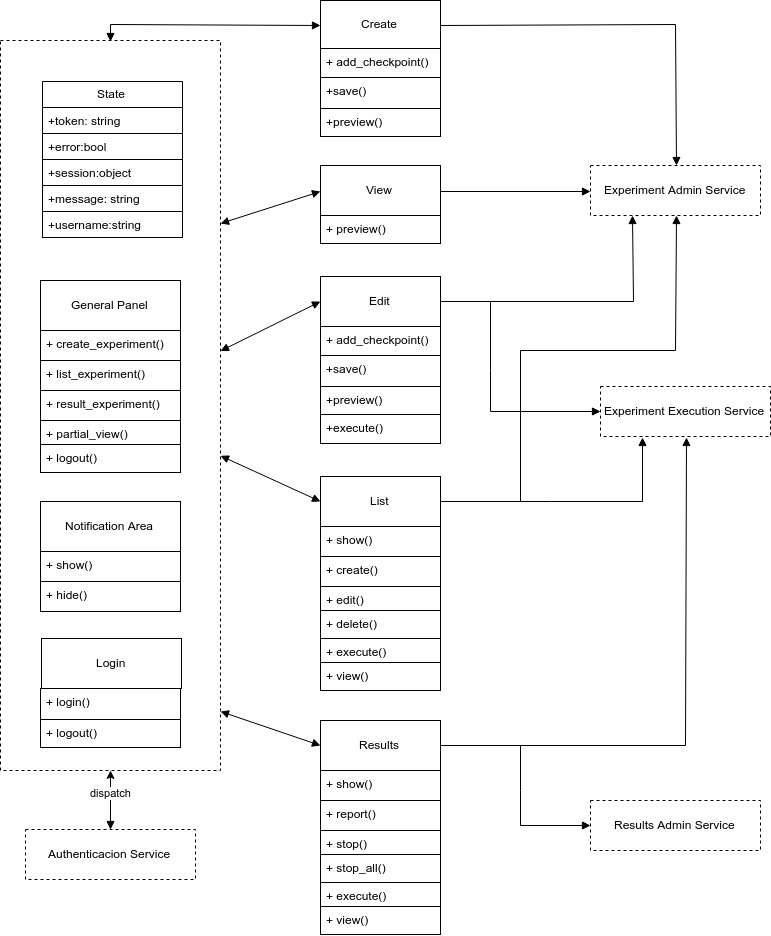
\includegraphics[scale=0.42]{../figures/d21.jpg}
    \caption{Arquitectura de la Interfaz Gr\'afica. }
    \label{fig:d21}
\end{figure}

La \textit{Interfaz Gr\'afica} esta implementada bajo directrices de ReactJs\cite{react_thinking}, donde
cada vista es una clase din\'amica con su propio estado interno\cite{react_components} . El objeto destacado y trasversal
en todas las vistas es \textit{State}\cite{react_state} el cual contiene informacion requerida por el 
\textit{Servidor} tal como las cookies de usuario \'o como tambien el despliegue de notificaciones ante 
una respuesta de error a alguno de los servicios REST.   


\newpage